
\section{Theory}

This section provides a short introduction to relevant theory in orbital mechanics and propagation of uncertainties. The intended reader is someone with a technical background other than orbital mechanics or statistics, and the goal is to give a sufficient understanding of necessary concepts. 


\subsection{Orbital Mechanics}

The sections on orbital mechanics are mostly based on the book by Curtis \cite{Curtis2009}.

\subsubsection{Orbital Parameters}

The following is an introduction to a parametric description of orbits, using the definitions from Curtis \cite{Curtis2009}. Under the assumption that an orbit is an ideal Keplerian orbit, it can be uniquely identified using six orbital elements. Three parameters are required to define the orbit on a plane, and three additional parameters are needed to further place the orbit in three dimensional space. \\

The three parameters used to describe an orbit on a plane are the \textit{specific angular momentum}, \textit{eccentricity}, and \textit{true anomaly}. The specific angular momentum is, as the name suggests, the angular momentum of the orbiting object. This value is constant at any point on a given orbit. The eccentricity value describes how much the shape of the orbit deviates from a circle, and can be found by dividing the distance between the center of the orbit and one of the foci by the \textit{semi-major axis} (longest distance to the central body). The shape of a orbit corresponding to different eccentricity values is given in Table \ref{table:eccentricity}. The true anomaly is the angle between the position of the orbiting object and \textit{periapsis} (the shortest distance to the central body). \\

\begin{table}[h]
\centering
\begin{tabular}{@{}ll@{}}
\toprule
$e = 0$      & Circle    \\
$0 < e < 1 $ & Ellipse   \\
$e = 1$      & Parabola  \\
$e > 1 $     & Hyperbola \\
\bottomrule
\end{tabular}
\caption{Orbital shapes for different eccentricity values}
\label{table:eccentricity}
\end{table}


To place the orbit in three dimensional space, three axis rotations are required. The orbital elements corresponding to these rotations are the \textit{inclination}, \textit{right ascension of the ascending node} and the \textit{argument of perigee}. The inclination describes the angle between the orbital plane and the \textit{equatorial} (Earth XY) plane. The right ascension of the ascending node is the angle between the equatorial X-axis and the point on the equatorial plane where the orbit passes through from below. The third angle, argument of perigee, is the angle in the orbital plane between the point the orbit passes above the equatorial plane and the point of perigee. \\


A summary of the six orbital elements is given in Table \ref{table:orbital_parameters}. \\


\begin{table}[h]
\centering
\begin{tabular}{@{}llll@{}}
\toprule
%\multicolumn{4}{c}{Orbital Parameters}                            \\ \midrule
Name                                  & Symbol              & Range     & Unit \\ \midrule
Specific angular momentum             & \textit{h}          & -         & $\frac{kgm}{s^2}$ \\
Inclination                           & \textit{i}          & [0, 180]  & Deg    \\
Right ascension of the ascending node & $\mathit{\Omega}$   & [0, 360]  & Deg  \\
Eccentricity                          & \textit{e}          & -         & -    \\
Argument of perigee                   & $\mathit{\omega}$   & [0, 360]  & Deg  \\
True anomaly                          & $\mathit{\Theta}$   & [0, 360]  & Deg  \\ \bottomrule
\end{tabular}
\caption{Overview of the six orbital parameters}
\label{table:orbital_parameters}
\end{table}


\subsubsection{Coordinate Systems}

\paragraph{Perifocal Coordinate System} 
The center of the perifocal coordinate system is at the focus of the orbit. The perifocal frame is defined with the unit vectors $\hat{\mathbf{p}}$, $\hat{\mathbf{q}}$ and $\hat{\mathbf{w}}$. The unit vectors $\hat{\mathbf{p}}$ and $\hat{\mathbf{q}}$ lie in the orbital plane, with $\hat{\mathbf{p}}$ pointing towards the \textit{periapsis} of the orbit and $\hat{\mathbf{q}}$ towards the point at which \textit{true anomaly} is equal to $90 \deg$. The unit vector $\hat{\mathbf{w}}$ is the cross product of the unit vectors in the orbital plane, $\hat{\mathbf{w}} = \hat{\mathbf{p}} \times \hat{\mathbf{q}}$, and thus points in the same direction as the angular momentum vector $\Vec{\mathbf{h}}$ of the orbiting object. \\

The position of the orbiting object described in the perifocal plane is given in Eq. \ref{eq:radius_perifocal_frame}, and velocity in Eq. \ref{eq:velocity_perifocal_frame}.

\begin{equation}
    \Vec{\mathbf{r}} = \Bar{x}\hat{\mathbf{p}} + \Bar{y}\hat{\mathbf{q}}
    \label{eq:radius_perifocal_frame}
\end{equation}

\begin{equation}
    \Vec{\mathbf{v}} = \dot{\Vec{\mathbf{r}}} = \dot{\Bar{x}}\hat{\mathbf{p}} + \dot{\Bar{y}}\hat{\mathbf{q}}
    \label{eq:velocity_perifocal_frame}
\end{equation}


\paragraph{Local Vertical Local Horizontal Coordinate System} 

Define the Local Vertical Local Horizontal (LVLH) coordinate frame. \\  
\todo{Fill in}

\paragraph{Earth Centered Intertial Coordinate System} 

Define the Earth Centered Intertial (ECI) coordinate frame. \\
\todo{Fill in}


\subsubsection{Lagrange Coefficients}

Using the Lagrange Coefficients, the functions \textit{f} and \textit{g}, from the French mathematical physicist Joseph-Louis Lagrange (1736-1813), we are able to describe the position and velocity of an orbiting object at any point in time if the initial conditions are known, as shown in Eq. \ref{eq:radius_lagrange_coefficients}. The Lagrange Coefficients are derived based on the fact that the angular momentum is constant throughout the orbit.   


\begin{equation}
    \Vec{\mathbf{r}} = f \Vec{\mathbf{r_0}} + g \Vec{\mathbf{v_0}}
    \label{eq:radius_lagrange_coefficients}
\end{equation}

The Lagrange Coefficients $f$ and $g$, and their time derivatives $\dot{f}$ and $\dot{g}$, are defined below.

\begin{align}
    f &= \frac{ \Bar{x} \dot{\Bar{y_0}} - \Bar{y} \dot{\Bar{x_0}} }{ h }
    \label{eq:lagrange_f} \\
    g &= \frac{ - \Bar{x} \Bar{y_0} + \Bar{y} \Bar{x_0} }{ h } 
    \label{eq:lagrange_g} \\
    \dot{f} &= \frac{ \dot{\Bar{x}} \dot{\Bar{y_0}} - \dot{\Bar{y}} \dot{\Bar{x_0}} }{ h } 
    \label{eq:lagrange_f_dot} \\
    \dot{g} &= \frac{ - \dot{\Bar{x}} \Bar{y_0} + \dot{\Bar{y}} \Bar{x_0} }{ h } 
    \label{eq:lagrange_g_dot}
\end{align}

Using the change in true anomaly $\Delta \Theta$, or the change in universal anomaly $\chi$, the Lagrange Coefficients and their time derivatives have the following expressions. The left column in the functions below are the expressions based on true anomaly $\Delta \Theta$, and the right column are the expressions based on universal anomaly $\chi$.

\begin{align}
    f &= 1 - \frac{ \mu r }{ h^2 } ( 1 - \cos{\Delta \Theta} ) &&= 1 - \frac{\chi^2}{r} C(z)
    \label{eq:lagrange_anomaly_f} \\
    g  &= \frac{ r_0 r }{ h } \sin{\Delta \Theta} &&= \Delta t - \frac{1}{\sqrt{\mu} \chi^3 S( z )}
    \label{eq:lagrange_anomaly_g} \\
    \dot{f} &= \frac{\mu}{h} \frac{1 - \cos{\Delta \Theta}}{\sin{\Delta \Theta}} [ \frac{\mu}{h^2} (1 - \cos{\Delta \Theta} - \frac{1}{r_0} - \frac{1}{r} ] &&= \frac{\sqrt{\mu}}{r_0 r} \chi [z S(z) - 1]
    \label{eq:lagrange_anomaly_f_dot} \\
    \dot{g} &= 1 - \frac{\mu r_0}{h^2} (1 - \cos{\Delta \Theta} ) &&= 1 - \frac{\chi^2}{r} C(z)
    \label{eq:lagrange_anomaly_g_dot}
\end{align}

For the functions above, $z = \alpha \chi^2$, $\alpha = \frac{1}{a}$ is the reciprocal of the semimajor axis, and $C(z)$ and $S(z)$ are \textit{Stumpff functions} defined below.

\begin{align}
    C(z) &= \sum_{k = 0}^{\infty} (-1)^k \frac{z^k}{(2k + 2)!} \\
    S(z) &= \sum_{k = 0}^{\infty} (-1)^k \frac{z^k}{(2k + 3)!}
\end{align}{}




\subsubsection{Lambert's problem}

Lambert's problem, from the French-born German astronomer J. H. Lambert (1728-1777), concerns finding the trajectory joining two orbital points $P_0$ and $P$, given the transfer time $\Delta t$.  \\

Algorithm \ref{algo:lambert} presents an approach using the Lagrange Coefficients to solve Lambert's problem. The methos presented is based on \textit{Algorithm 5.2} from the book by Curtis \cite{Curtis2009}.

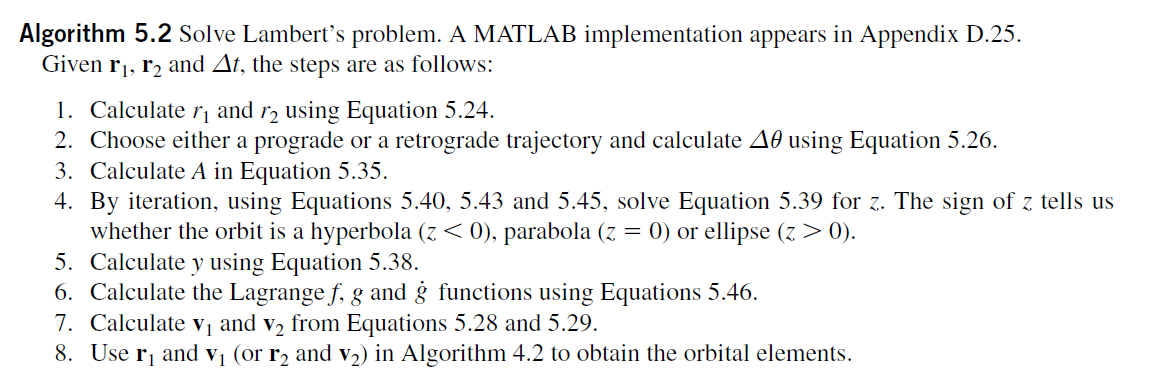
\includegraphics[width=\textwidth]{Images/Alg52.PNG}

\begin{algorithm}
    \setstretch{1.2}
    \DontPrintSemicolon
    \KwIn{Starting point, end point, direction and time frame of desired trajectory}
    \KwOut{Initial velocity required to follow desired trajectory and velocity at end point}
    Calculate the change in true anomaly, $\mathit{\Delta\Theta}$, based on starting point, end point and direction of orbit (prograde or retrograde)\;
    \Return{velocityStart, velocityEnd}\;
    \caption{Solve Lambert's Problem Using Lagrange Coefficients}
    \label{algo:lambert}
\end{algorithm}

\todo{Insert Algorithm from Curtis}



%%%%%%%%%%%%%%%%%%%%%%%%%%%%%%%%%%%%%%%%%%%%%%%%%%%%%%%%%%%%%%%%


\subsection{Uncertainty Propagation}

In the following section different methods of uncertainty propagation are presented. The term \textit{uncertainty propagation} refers to the method of predicting a systems state and associated uncertainty at a certain point in time, given information about the initial state and uncertainty of the system. A propagator can be either linear or nonlinear, with several approaches existing within both classes. \\


\subsubsection{Monte Carlo Simulations}

Monte Carlo simulation relies on repeated random sampling to obtain numerical results. MC simulation is computationally heavy, but has the advantage that when the number of samples approaches infinity, the result converges towards the true probability distribution of the system. \\


